\section{Paper-specific project}\label{sec:project}
In this section, we compare two of the data fission procedures introduced in \cite{leiner2022data} for Gaussian distributed data against data splitting, in the context of constructing selective CIs in fixed-design linear regression models. Suppose we are given a set of $n$ observations such that for $i\in\{1,\dots,n\}$, $y_i = x_i^\top \beta + \eps_i$,
where for some $p\in\nats$ and known $\sigma>0$, $x_i\in\reals^p$, $\eps_i\distiid \distNorm(0,\sigma^2)$, $\beta\in\reals^p$. Equivalently, we can write $Y_i\distas\distNorm(x_i^\top\beta, \sigma^2)$. Note here we assume that the covariates $x_i$'s are fixed. The goal is to first perform variable selection and then construct CIs for the regression coefficients corresponding to the selected variables. We would like to compare variable selection accuracy as well as inference quality obtained using the following three procedures:
\begin{itemize}
\item Data fission (P1): for each $i\in\{1,\dots,n\}$, and some fixed $\tau\in(0,\infty)$, draw $Z_i\distas\distNorm(0,\sigma^2)$. Let $f_\tau(Y_i) = Y_i + \tau Z_i$, $g_\tau(Y_i) = Y_i - \tau^{-1}Z_i$. Then $f_\tau(Y_i)\indep g_\tau(Y_i)$ and $f_\tau(Y_i)\distas\distNorm(x_i^\top\beta, (1+\tau^2)\sigma^2)$, $g_\tau(Y_i)\distNorm(x_i^\top\beta, (1+\tau^{-2})\sigma^2)$. We use $(f_\tau(Y_i))_{i=1}^n$ for selection and $(g_\tau(Y_i))_{i=1}^n$ for inference.
\item Data fission (P2): for each $i\in\{1,\dots,n\}$, and some fixed $\tau\in(0,\infty)$, draw $Z_i\distas\distNorm(Y_i,\tau\sigma^2)$. Let $f_\tau(Y_i) = Z_i$, $g_\tau(Y_i) = Y_i$. Then $f_\tau(Y_i)\distas\distNorm(x_i^\top\beta, (1+\tau)\sigma^2)$, $g_\tau(Y_i)\given f_\tau(Y_i)\distas\distNorm\left(\frac{\tau}{\tau+1}x_i^\top\beta + \frac{1}{\tau+1}f_\tau(Y_i), \frac{\tau}{\tau+1}\sigma^2\right)$. We use $(f_\tau(Y_i))_{i=1}^n$ for selection and $(g_\tau(Y_i))_{i=1}^n$ for inference.
\item Data splitting: for some fixed $a\in\{\frac{1}{n}, \frac{2}{n}, \dots, 1\}$, randomly draw $an$ observations from $(Y_i)_{i=1}^n$ without replacement. Without loss of generality, denote the first $an$ observations as those that are selected. Use $(Y_i)_{i=1}^{an}$ for selection and $(Y_i)_{i=an+1}^n$ for inference.
\end{itemize}
We begin by observing the three datasets used for the selection step. Both data fission procedures inflate the variance of each observation without changing their underlying means. Data splitting, on the other hand, directly reduces the number of observations without perturbing their underlying distributions. This also introduces uncertainty to the selection step. It is then of interest to compare variable selection accuracies under different sample sizes and the amount of variance inflated. However, recall that from the Fisher information perspective, to make the comparison fair, we set $a = \frac{1}{1+\tau^2}$. As a result, the comparison reduces to be about varying the sample sizes.

We now consider the inference stage. Suppose that the selected model is $M\subset\{1,\dots,p\}$ and that
\[
X_M = \begin{bmatrix} x_{M,1}, \dots, x_{M,n} \end{bmatrix}^\top, \quad Y = \begin{bmatrix} Y_1, \dots, Y_n \end{bmatrix}^\top,
\]
where $x_{M,i}$ is a vector consisting of only the covariates corresponding to the selected features. We then have our ideal target parameter given $M$ as
\[
\beta^\star(M) = \argmin_{\tilde{\beta}} \EE_Y \|Y - X_M\tilde{\beta}\|^2 = (X_M^\top X_M)^{-1}(X_M^\top\mu)
\]
where $\mu = \begin{bmatrix} x_1^\top\beta, \dots, x_n^\top\beta \end{bmatrix}^\top$. However, since we are using slightly perturbed datasets for inference, our estimator $\hbeta(M)$ given the model $M$ for each of the three procedures are
\begin{itemize}
\item Data fission (P1): $\hbeta(M) = (X_M^\top X_M)^{-1}X_M^\top g_\tau(Y) \distas \distNorm(\beta^\star(M), \sigma^2(1+\tau^{-2})(X_M^\top X_M)^{-1})$;
\item Data fission (P2):\\ $\hbeta(M) = (X_M^\top X_M)^{-1}X_M^\top g_\tau(Y) \given f_\tau(Y) \distas \distNorm(\frac{\tau}{\tau+1}\beta^\star(M) + \frac{1}{\tau+1}(X_M^\top X_M)^{-1}X_M^\top f(Y), \sigma^2\frac{\tau}{\tau+1}(X_M^\top X_M)^{-1})$;
\item Data splitting: $\hbeta(M) = (X_M^\top X_M)^{-1}X_M^\top Y \distas \distNorm(\beta^\star(M), \sigma^2(X_M^\top X_M)^{-1})$.
\end{itemize}
Note that here $f$ and $g$ are applied to each entry of $Y$ and that $X_M$ and $Y$ in data splitting only contains a subset set of $na$ observations.

Looking at the means of each estimator above, both the data fission (P1) and data splitting procedures target $\beta^\star(M)$. On the other hand, the mean of the data fission (P2) estimator depends on the realized values of the external random variable $Z$. Since $\EE[f_\tau(Y)] = \mu$, if we marginalize $f_\tau(Y)$ over the distribution of $\hbeta(M)$, data fission (P2) would also target the ideal parameter $\beta^\star(M)$. However, it is reasonable to suspect that this randomness might affect the quality of inference.

We now look at the variances of the three estimators. Similar to the selection stage, data fission (P1) inflates the variance of $\hbeta(M)$ by a function of $\tau$, and data splitting introduces additional uncertainty by reducing the sample size. However, in data fission (P2), the variance is deflated. Suppose for each $i$, $x_i$ is generated (\iid) by some distribution $\pi$, and assume that for all selected model $M$, $\EE[x_{M,1}x_{M,1}^\top]$ is finite and strictly positive. Then we have
\[
\frac{1}{n}X_M^\top X_M \convp \EE[x_{M,1}x_{M,1}^\top] \implies \left(\frac{1}{n}X_M^\top X_M\right)^{-1} \convp \left( \EE[x_{M,1}x_{M,1}^\top] \right)^{-1} \implies X_M^\top X_M \convp \frac{1}{n}\left( \EE[x_{M,1}x_{M,1}^\top] \right)^{-1}.
\]
Under this assumption, the difference in inference between data splitting and data fission once again comes down to the sample size and the amount of variance inflated or deflated by $\tau$. We therefore set up our simulations as following. Note that this is mostly in line with Section 4 of \cite{leiner2022data}.

We set $a = \frac{1}{2}$ and $\tau=1$ to ensure the amount of Fisher information allocated to the selection stage is the same across all three methods. Let $p=20, \beta_1=\beta_{19}=1$, $\beta_2=\beta_{20}=-1$, and the rest of the entries in $\beta$ be $0$. We also generate the covariates from the standard multivariate Guassian distribution. Note that there is no intercept in our regression model. We then conduct selective inference with varying sample sizes $10, 20, 50, 100$ to evaluate how the performances across all three methods change under different sample sizes. To compare variable selection accuracy, we use as our metrics
\[
\text{power} = \frac{|j\in M: \beta_j \neq 0|}{|j\in [p]: \beta_j \neq 0|}, \quad \text{precision} = \frac{|j\in M: \beta_j \neq 0|}{|M|}.
\]
To compare the quality of inference, we look at
\[
\text{FCR} = \frac{|k\in M: [\beta^\star(M)]_k \notin CI_k|}{\max{|M|, 1}}, \quad \overline{\text{CI len.}} = \frac{\sum_{k\in M} |CI_k(2) - CI_k(1)|}{|M|}, \quad \text{L2 err.} = \frac{\| \beta^\star(M) - \hbeta(M) \|_2^2}{|M|}.
\]
To perform variable selection, we use the \texttt{glmnet} package in \texttt{R} with the default settings with the regularization parameter set to \texttt{lambda.1se}. We repeat the above experiments $200$ times and report the median of the above metrics (excluding runs that do not end up selecting any variable in the selection step) in \cref{fig:median}. The same set of plots with the IQR of each metric is included in \cref{apdx:plots}. Note that since the IQRs have a lot of overlaps, the discussion below is only concerned with the average performance rather than individual trials. The code used to run the simulations and generate the plots can be found at \url{https://github.com/NaitongChen/QP-3}.

\captionsetup[subfigure]{labelformat=empty}
\begin{figure}[ht!]
\centering
\begin{subfigure}[b]{.32\columnwidth} 
    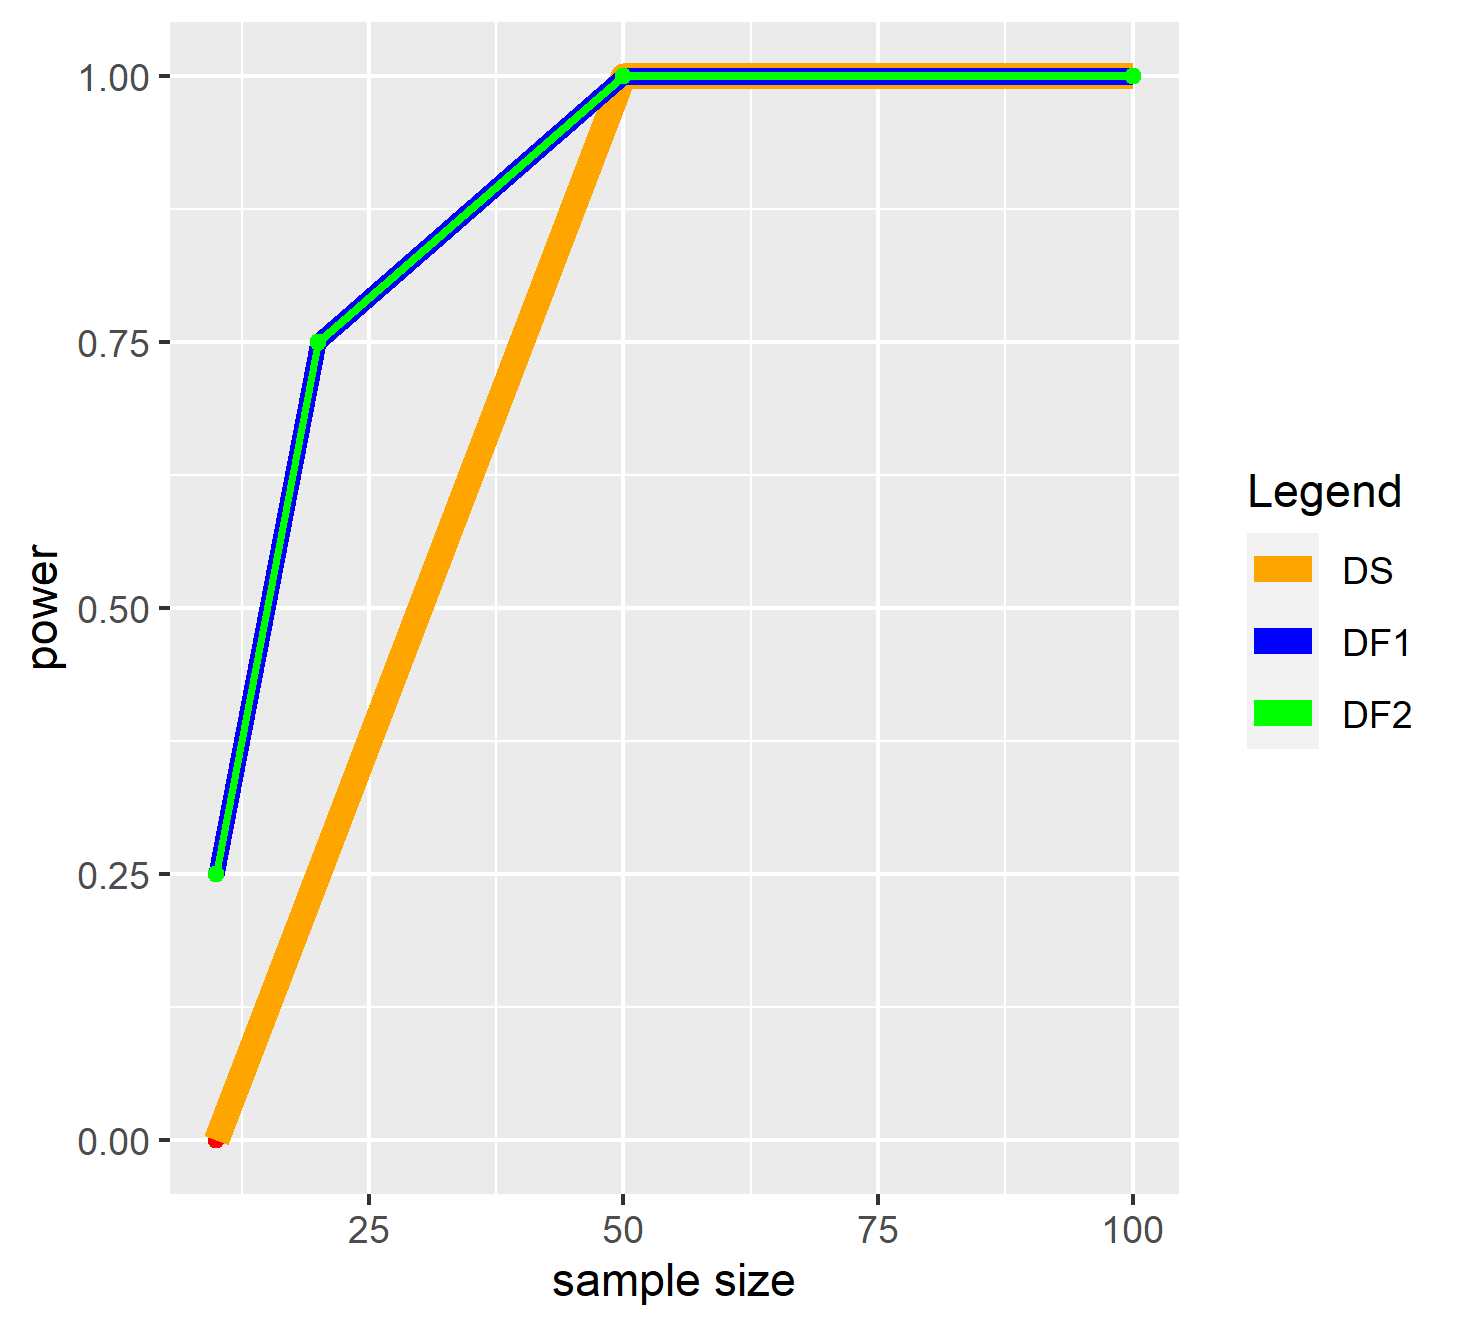
\includegraphics[width=\columnwidth]{../../plot/power_1.png}
    \caption{(a) power}
\end{subfigure}
\hfill
\centering
\begin{subfigure}[b]{.32\columnwidth} 
    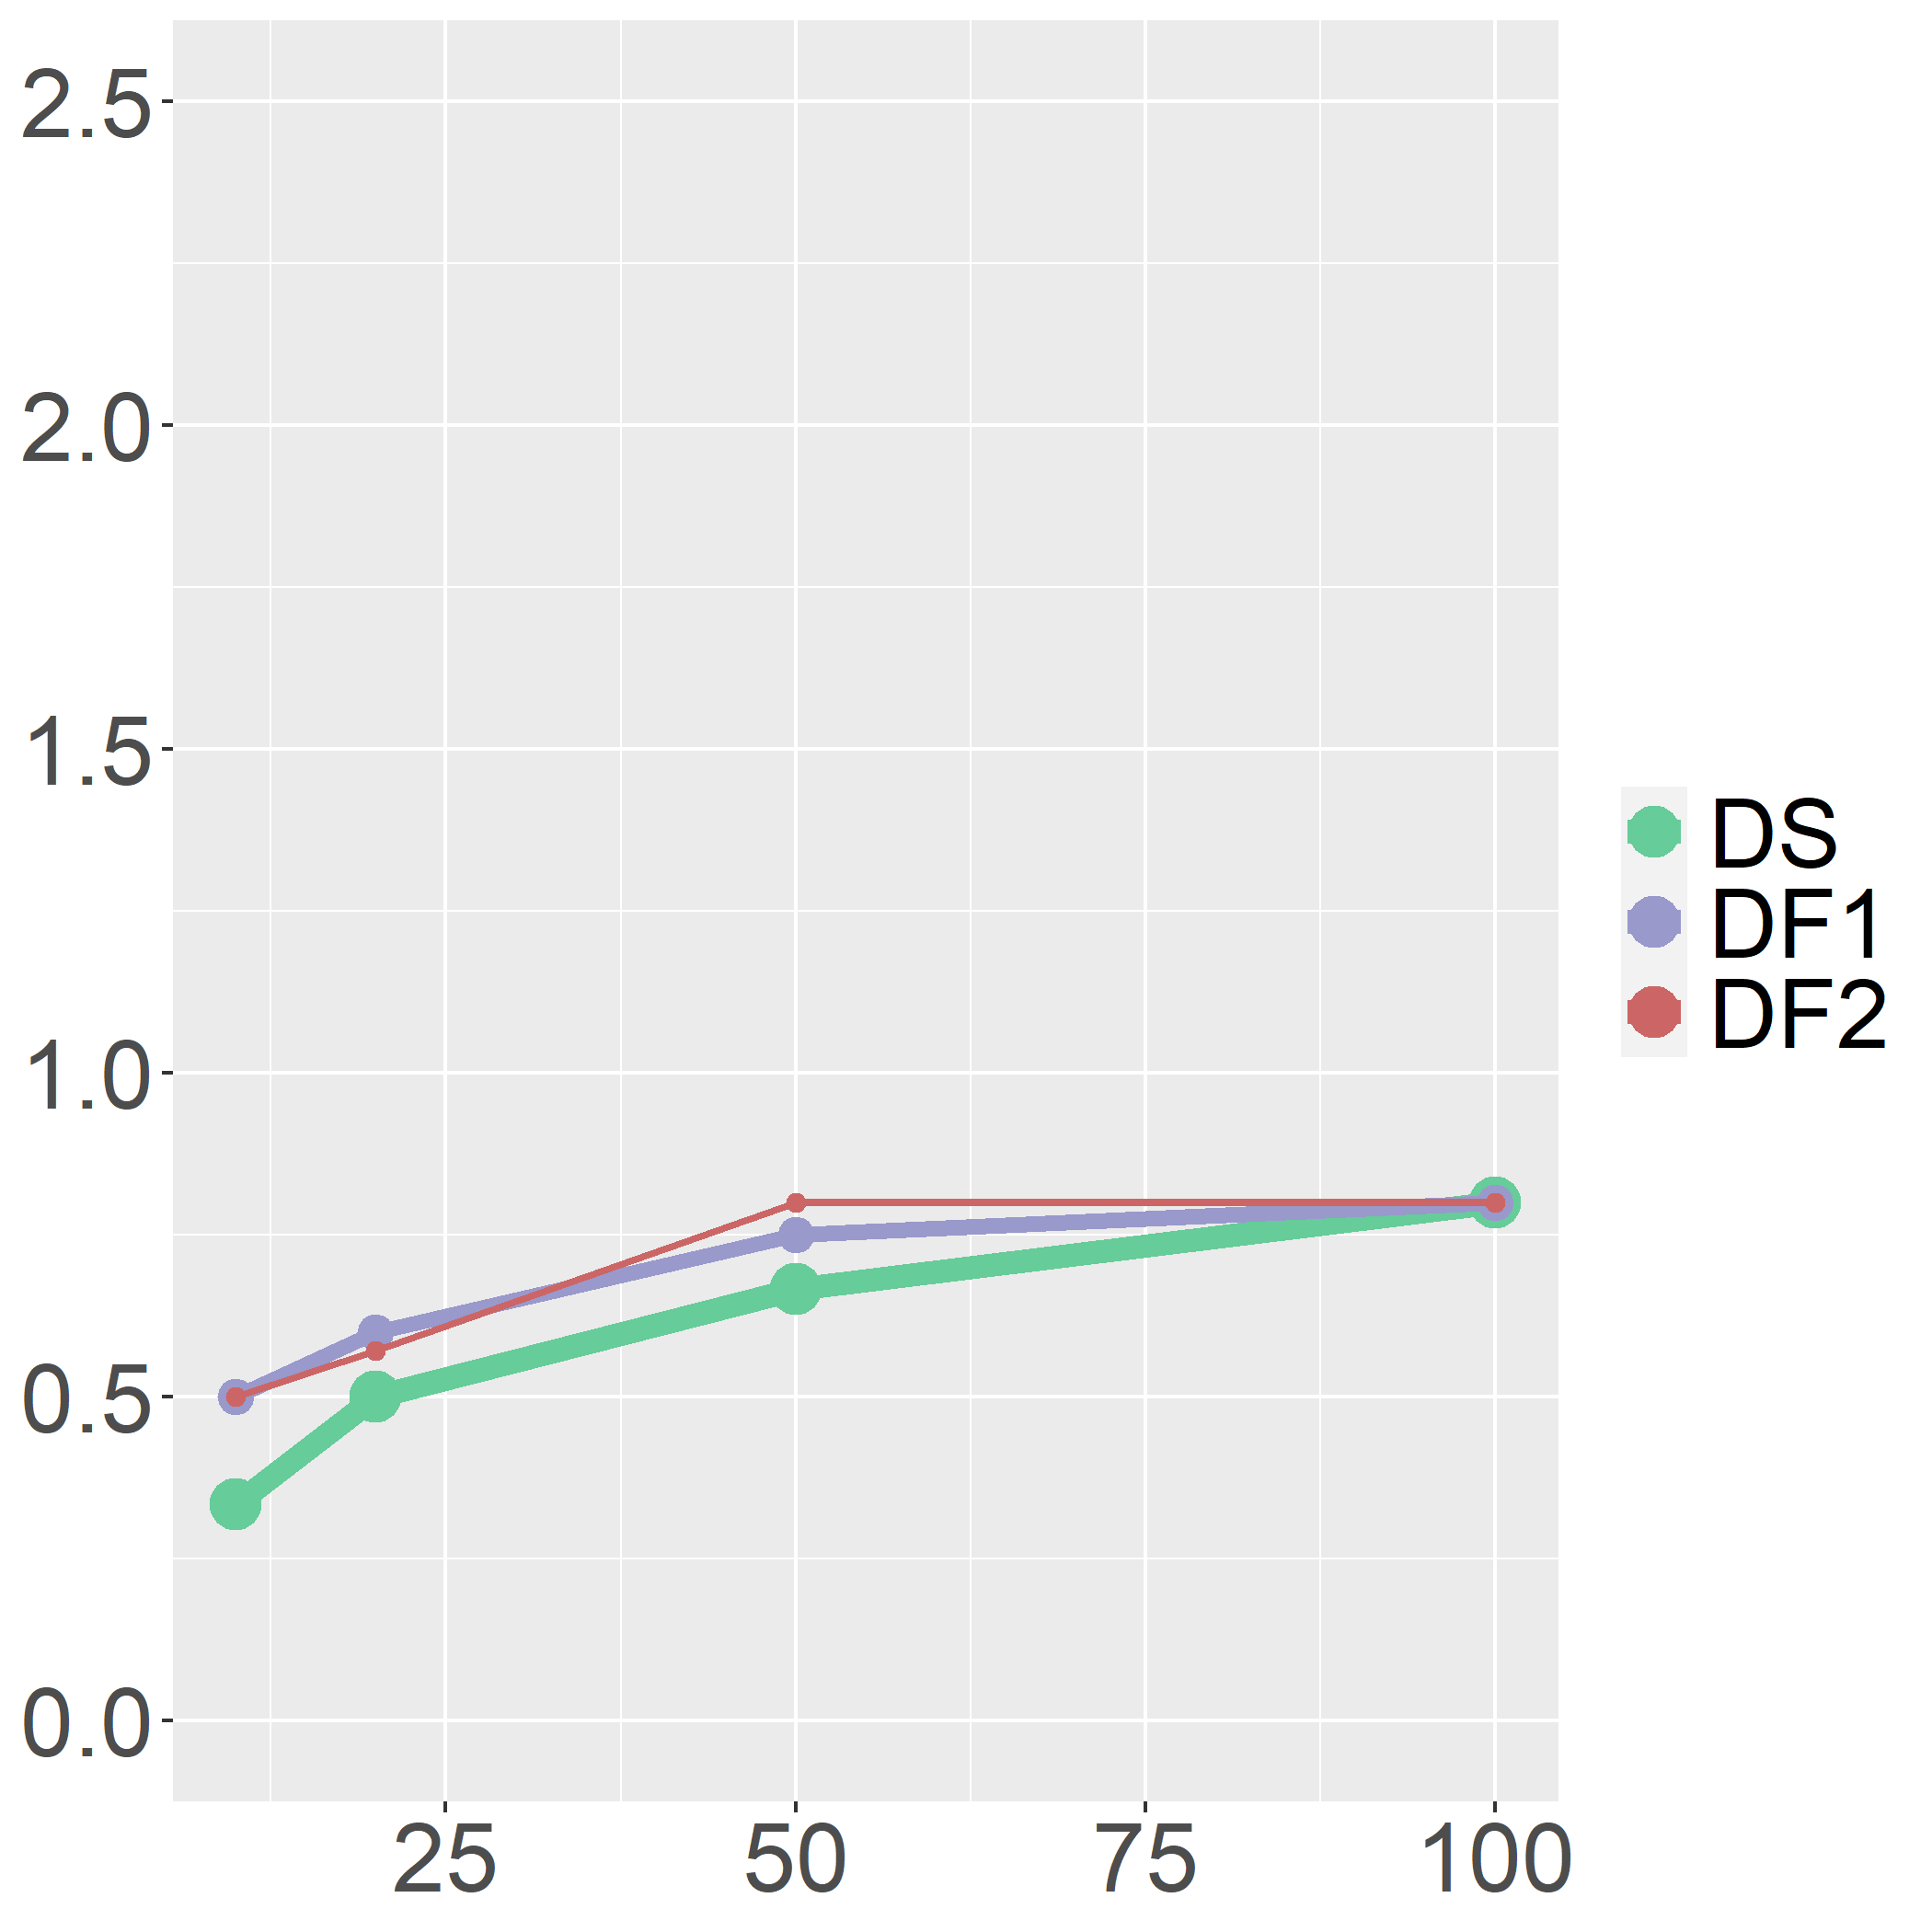
\includegraphics[width=\columnwidth]{../../plot/precision_1.png}
    \caption{(b) precision}
\end{subfigure}
\\
\centering
\begin{subfigure}[b]{.32\columnwidth} 
    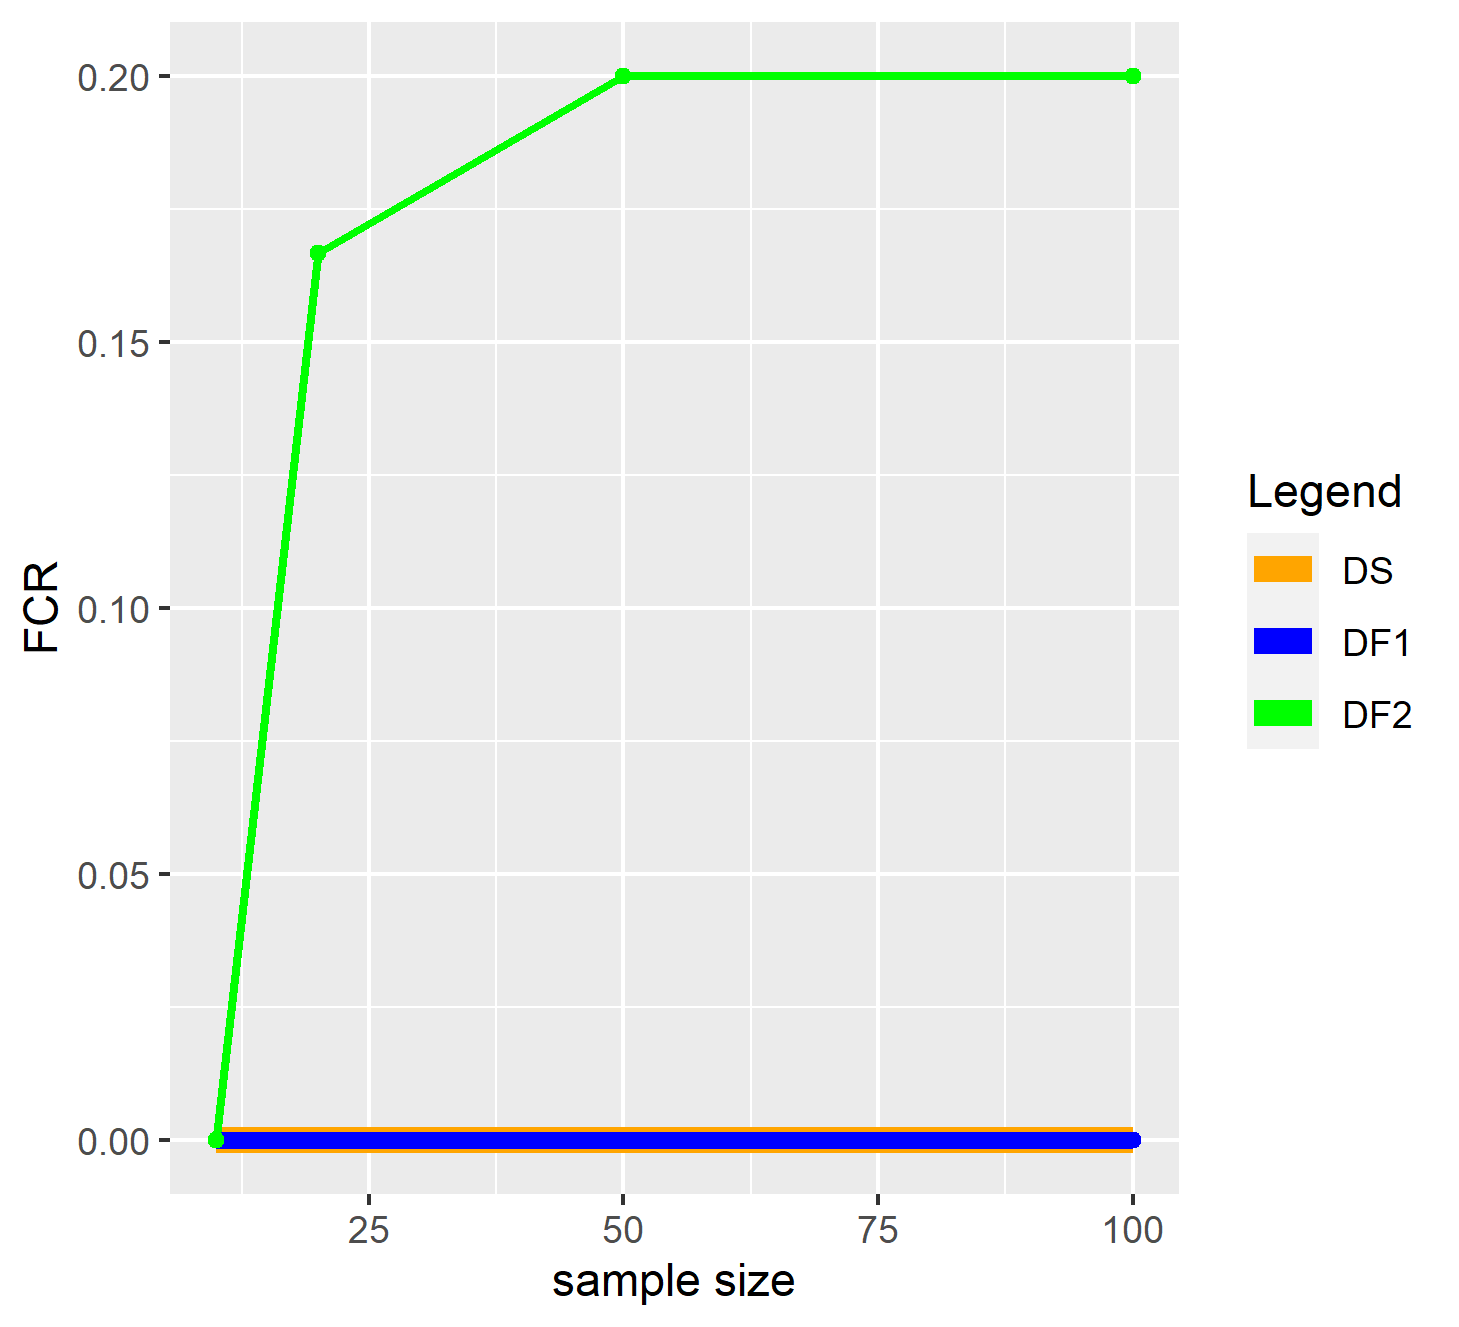
\includegraphics[width=\columnwidth]{../../plot/FCR_1.png}
    \caption{(c) FCR}
\end{subfigure}
\hfill
\centering
\begin{subfigure}[b]{.32\columnwidth} 
    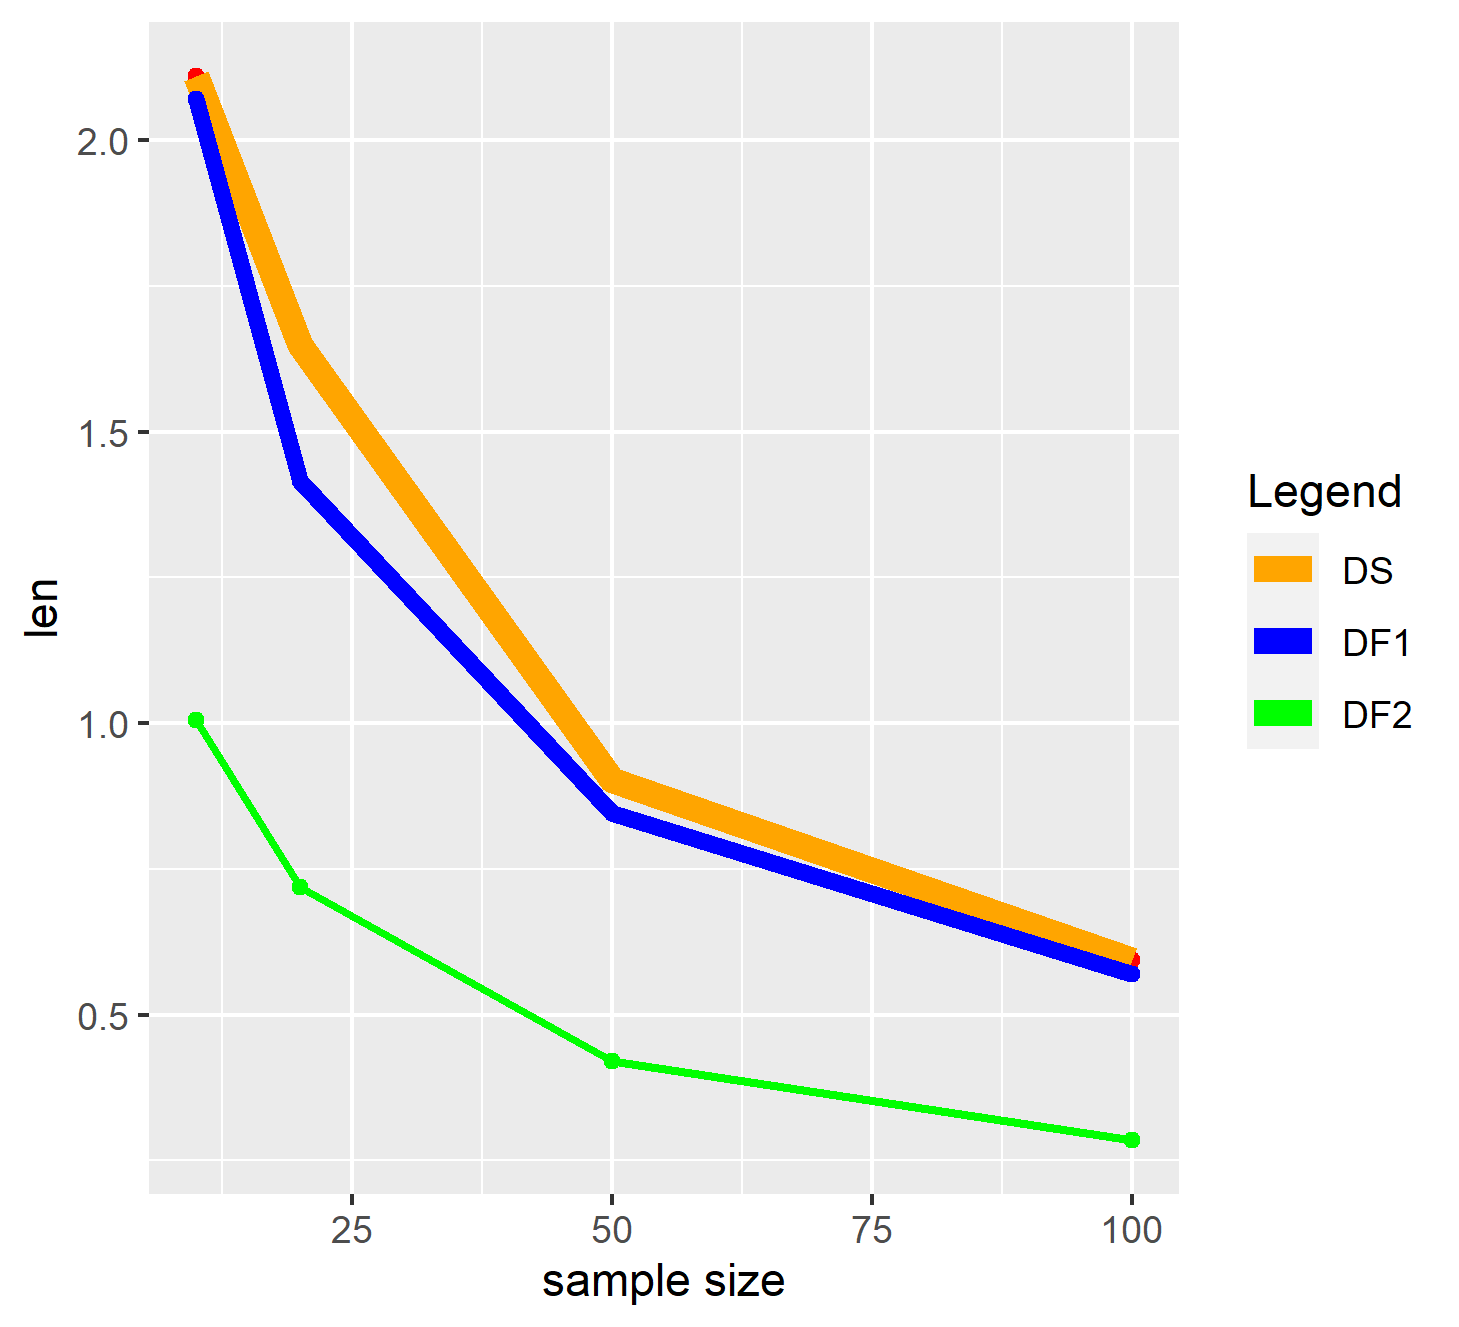
\includegraphics[width=\columnwidth]{../../plot/len_1.png}
    \caption{(d) Average CI length}
\end{subfigure}
\hfill
\centering
\begin{subfigure}[b]{.32\columnwidth} 
    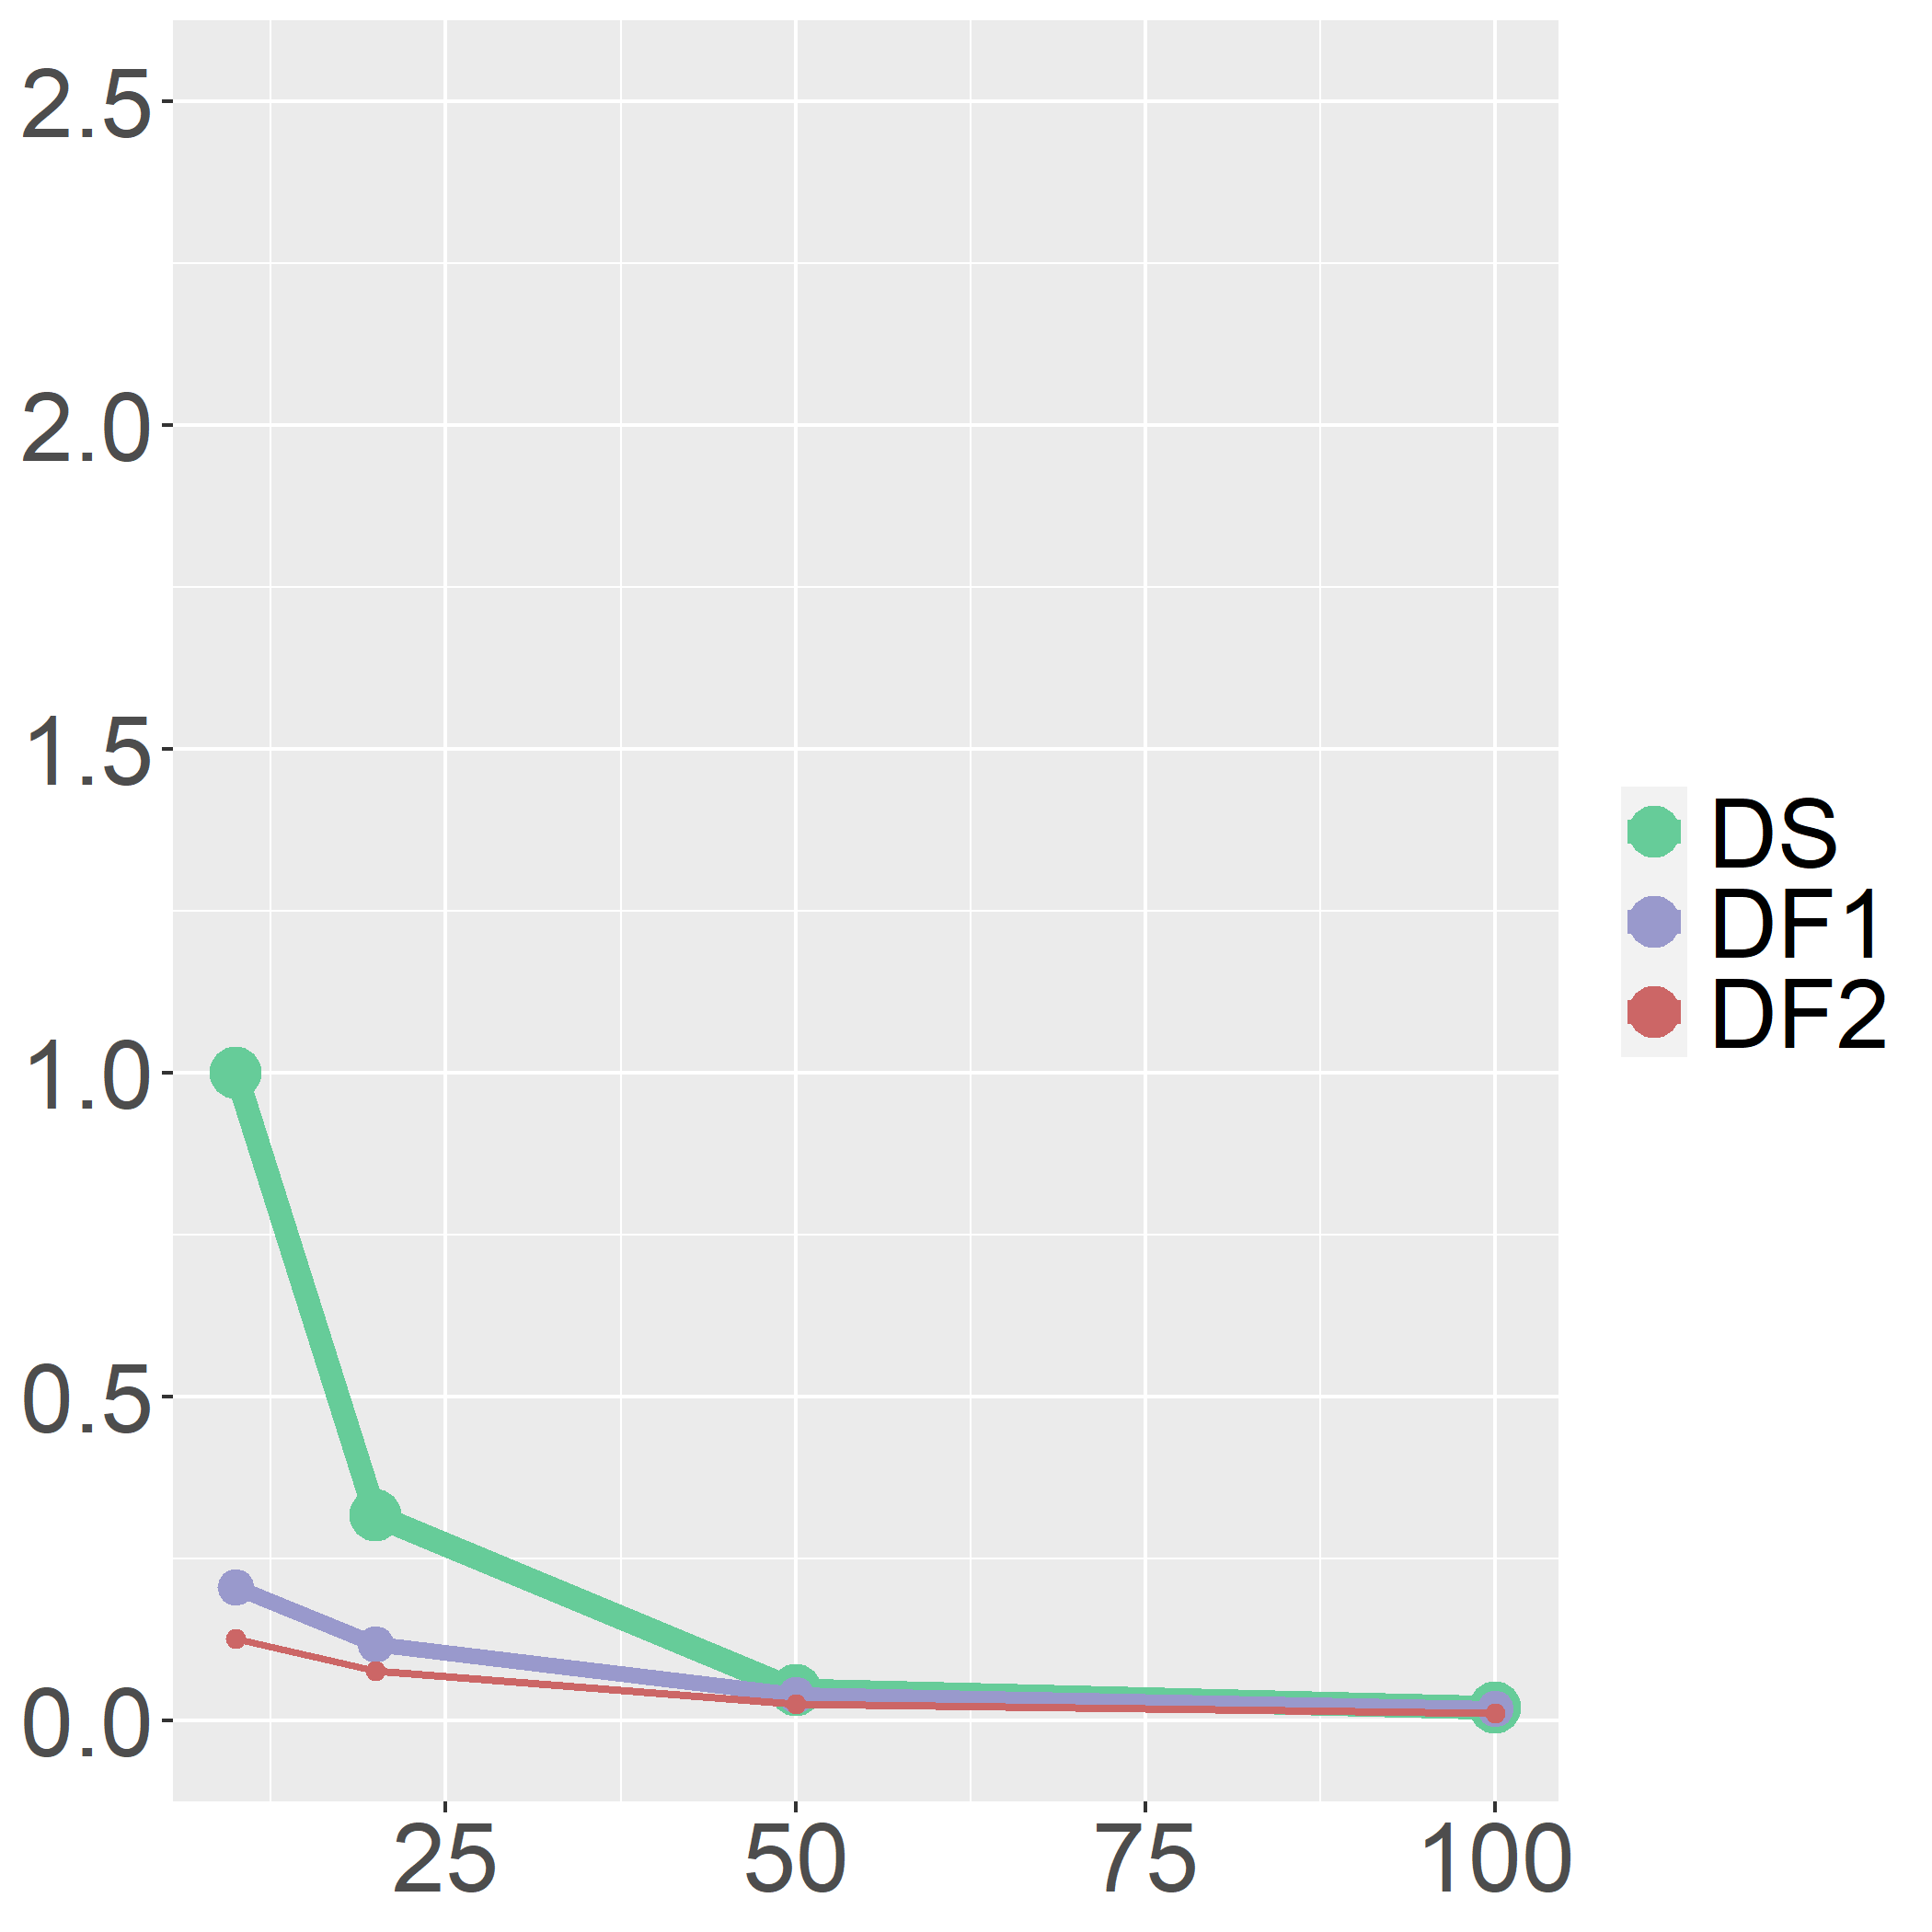
\includegraphics[width=\columnwidth]{../../plot/L2_1.png}
    \caption{(e) L2 error}
\end{subfigure}
\hfill
\caption{caption}
\label{fig:median}
\end{figure}

-------------------------------------------------------------------------------------------------------------------------------------

We begin by comparing variable selection accuracy. In particular we look at power and precision (give definition). Both power and precision are similar between the two data fission procedures, because they have the same $f(X)$ marginal distributions. Compared to data splitting, data fission achieves better power and precision particularly when sample size is small, although this difference wears off as sample size increases. When there are few observations, the consequence that data splitting only works with half of the observations becomes apparent. If we look at individual trials, data splitting tends to miss true features (low power) and pick instead many false features (low precision). When there is not a lot of information from the data, halving the number of observations hinders the quality of variable selection, which is to be expected. Although data fission inflates the variance of the observations (by a factor of 2), this is a worthy sacrifice when the sample size is small. As we increase the sample size, even half of the information becomes sufficient for variable selection, making the advantage of data fission less obvious.

We now look at the quality of inference. Here we look at false coverage rate (FCR), length of CIs, and the L2 error between the estimated parameter and the ideal target of inference.

Median FCR for data splitting and data fission p1 are both well below $\alpha = 0.05$ (No correction needed, cite data fission paper). On the other hand, data fission p2 has a much higher FCR. This is because P2 not targeting the right beta star. In addition, having the CI se decrease does not help. Higher FCR could be that $(X^\top X)^-1$ converges, but randomness in $f(y)$ does not change. Worth noting that having low FCR does not necessarily mean we recover the true parameters, because there is a discrepancy between true and targeted beta's, especially when sample size is small.

Length of CI: P2 smaller than the other two. P1 and splitting are similar. P1 and splitting similar, probably because halving data and inflated variance cancel each other out. P2 has smaller length because variance smaller and sample size doesn't change.

L2 error decays by the variance of beta hat. Data splitting is worse because halving data. Obvious when sample size is small, and less so when sample size is large. Similarities between P1 and P2 somewhat surprising. might need to inflate sigma2 to make things clearer? Need further investigation.

Overall, in linear regression, P1 and splitting asymptotically similar, but P1 offering better performance when sample size is small, in both selection and inference. P2 is similar to P1 at selection, but inference performance is hindered by bias. To conclude, if we know variance, and have a small sample, use data fission over splitting. P1 better than P2 because no bias. Raises questions on how to deal with this randomness in P2, as it does give a framework for extending data fission to non Gaussian data.

Worth noting that these metrics appear to be highly variable. This implies that given a single instance of data fission vs. data splitting, the performance in terms of these metrics may be pretty similar, but on average, we observe the phenomenons discussed above.